%%
%% This is file `sample-sigconf.tex',
%% generated with the docstrip utility.
%%
%% The original source files were:
%%
%% samples.dtx  (with options: `sigconf')
%% 
%% IMPORTANT NOTICE:
%% 
%% For the copyright see the source file.
%% 
%% Any modified versions of this file must be renamed
%% with new filenames distinct from sample-sigconf.tex.
%% 
%% For distribution of the original source see the terms
%% for copying and modification in the file samples.dtx.
%% 
%% This generated file may be distributed as long as the
%% original source files, as listed above, are part of the
%% same distribution. (The sources need not necessarily be
%% in the same archive or directory.)
%%
%% The first command in your LaTeX source must be the \documentclass command.
\documentclass[sigconf]{acmart}
%% NOTE that a single column version may be required for 
%% submission and peer review. This can be done by changing
%% the \doucmentclass[...]{acmart} in this template to 
%% \documentclass[manuscript,screen]{acmart}
%% 
%% To ensure 100% compatibility, please check the white list of
%% approved LaTeX packages to be used with the Master Article Template at
%% https://www.acm.org/publications/taps/whitelist-of-latex-packages 
%% before creating your document. The white list page provides 
%% information on how to submit additional LaTeX packages for 
%% review and adoption.
%% Fonts used in the template cannot be substituted; margin 
%% adjustments are not allowed.
%%
%%
%% \BibTeX command to typeset BibTeX logo in the docs
\AtBeginDocument{%
  \providecommand\BibTeX{{%
    \normalfont B\kern-0.5em{\scshape i\kern-0.25em b}\kern-0.8em\TeX}}}

%% Rights management information.  This information is sent to you
%% when you complete the rights form.  These commands have SAMPLE
%% values in them; it is your responsibility as an author to replace
%% the commands and values with those provided to you when you
%% complete the rights form.
\setcopyright{acmcopyright}
\copyrightyear{2018}
\acmYear{2018}
\acmDOI{10.1145/1122445.1122456}

%% These commands are for a PROCEEDINGS abstract or paper.
% \acmConference[Woodstock '18]{Woodstock '18: ACM Symposium on Neural
%   Gaze Detection}{June 03--05, 2018}{Woodstock, NY}
% \acmBooktitle{Woodstock '18: ACM Symposium on Neural Gaze Detection,
%   June 03--05, 2018, Woodstock, NY}
% \acmPrice{15.00}
% \acmISBN{978-1-4503-XXXX-X/18/06}


%%
%% Submission ID.
%% Use this when submitting an article to a sponsored event. You'll
%% receive a unique submission ID from the organizers
%% of the event, and this ID should be used as the parameter to this command.
%%\acmSubmissionID{123-A56-BU3}

%%
%% The majority of ACM publications use numbered citations and
%% references.  The command \citestyle{authoryear} switches to the
%% "author year" style.
%%
%% If you are preparing content for an event
%% sponsored by ACM SIGGRAPH, you must use the "author year" style of
%% citations and references.
%% Uncommenting
%% the next command will enable that style.
%%\citestyle{acmauthoryear}

%%
%% end of the preamble, start of the body of the document source.
\begin{document}

%%
%% The "title" command has an optional parameter,
%% allowing the author to define a "short title" to be used in page headers.
\title{Super Duper Dataset for Experimental Analysis of CFPQ Algorithms}

%%
%% The "author" command and its associated commands are used to define
%% the authors and their affiliations.
%% Of note is the shared affiliation of the first two authors, and the
%% "authornote" and "authornotemark" commands
%% used to denote shared contribution to the research.
\author{Author 1}
\authornote{Both authors contributed equally to this research.}
\email{author_1@samplemail.com}
\orcid{1234-5678-9012}
\author{Author 2}
\authornotemark[1]
\email{author_2@samplemail.com}
\affiliation{%
  \institution{institution}
  \streetaddress{streetaddress}
  \city{city}
  \state{state}
  \country{country}
  \postcode{43017-6221}
}

\author{Author 3}
\email{author_3@samplemail.com}
\orcid{1234-5678-9012}
\affiliation{%
  \institution{institution}
  \streetaddress{streetaddress}
  \city{city}
  \state{state}
  \country{country}
  \postcode{43017-6221}
}

%%
%% By default, the full list of authors will be used in the page
%% headers. Often, this list is too long, and will overlap
%% other information printed in the page headers. This command allows
%% the author to define a more concise list
%% of authors' names for this purpose.
% \renewcommand{\shortauthors}{Trovato and Tobin, et al.}

%%
%% The abstract is a short summary of the work to be presented in the
%% article.
\begin{abstract}
  1 We introduce CFPQ\_Data dataset for super duper purposes.
  2 We introduce CFPQ\_Data dataset for super duper purposes.
  3 We introduce CFPQ\_Data dataset for super duper purposes.
  4 We introduce CFPQ\_Data dataset for super duper purposes.
  5 We introduce CFPQ\_Data dataset for super duper purposes.
  6 We introduce CFPQ\_Data dataset for super duper purposes.
  7 We introduce CFPQ\_Data dataset for super duper purposes.
  8 We introduce CFPQ\_Data dataset for super duper purposes.
\end{abstract}

%%
%% The code below is generated by the tool at http://dl.acm.org/ccs.cfm.
%% Please copy and paste the code instead of the example below.
%%
% \begin{CCSXML}
% <ccs2012>
%  <concept>
%   <concept_id>10010520.10010553.10010562</concept_id>
%   <concept_desc>Computer systems organization~Embedded systems</concept_desc>
%   <concept_significance>500</concept_significance>
%  </concept>
%  <concept>
%   <concept_id>10010520.10010575.10010755</concept_id>
%   <concept_desc>Computer systems organization~Redundancy</concept_desc>
%   <concept_significance>300</concept_significance>
%  </concept>
%  <concept>
%   <concept_id>10010520.10010553.10010554</concept_id>
%   <concept_desc>Computer systems organization~Robotics</concept_desc>
%   <concept_significance>100</concept_significance>
%  </concept>
%  <concept>
%   <concept_id>10003033.10003083.10003095</concept_id>
%   <concept_desc>Networks~Network reliability</concept_desc>
%   <concept_significance>100</concept_significance>
%  </concept>
% </ccs2012>
% \end{CCSXML}

% \ccsdesc[500]{Computer systems organization~Embedded systems}
% \ccsdesc[300]{Computer systems organization~Redundancy}
% \ccsdesc{Computer systems organization~Robotics}
% \ccsdesc[100]{Networks~Network reliability}

%%
%% Keywords. The author(s) should pick words that accurately describe
%% the work being presented. Separate the keywords with commas.
% \keywords{datasets, neural networks, gaze detection, text tagging}

%% A "teaser" image appears between the author and affiliation
%% information and the body of the document, and typically spans the
%% page.
% \begin{teaserfigure}
%   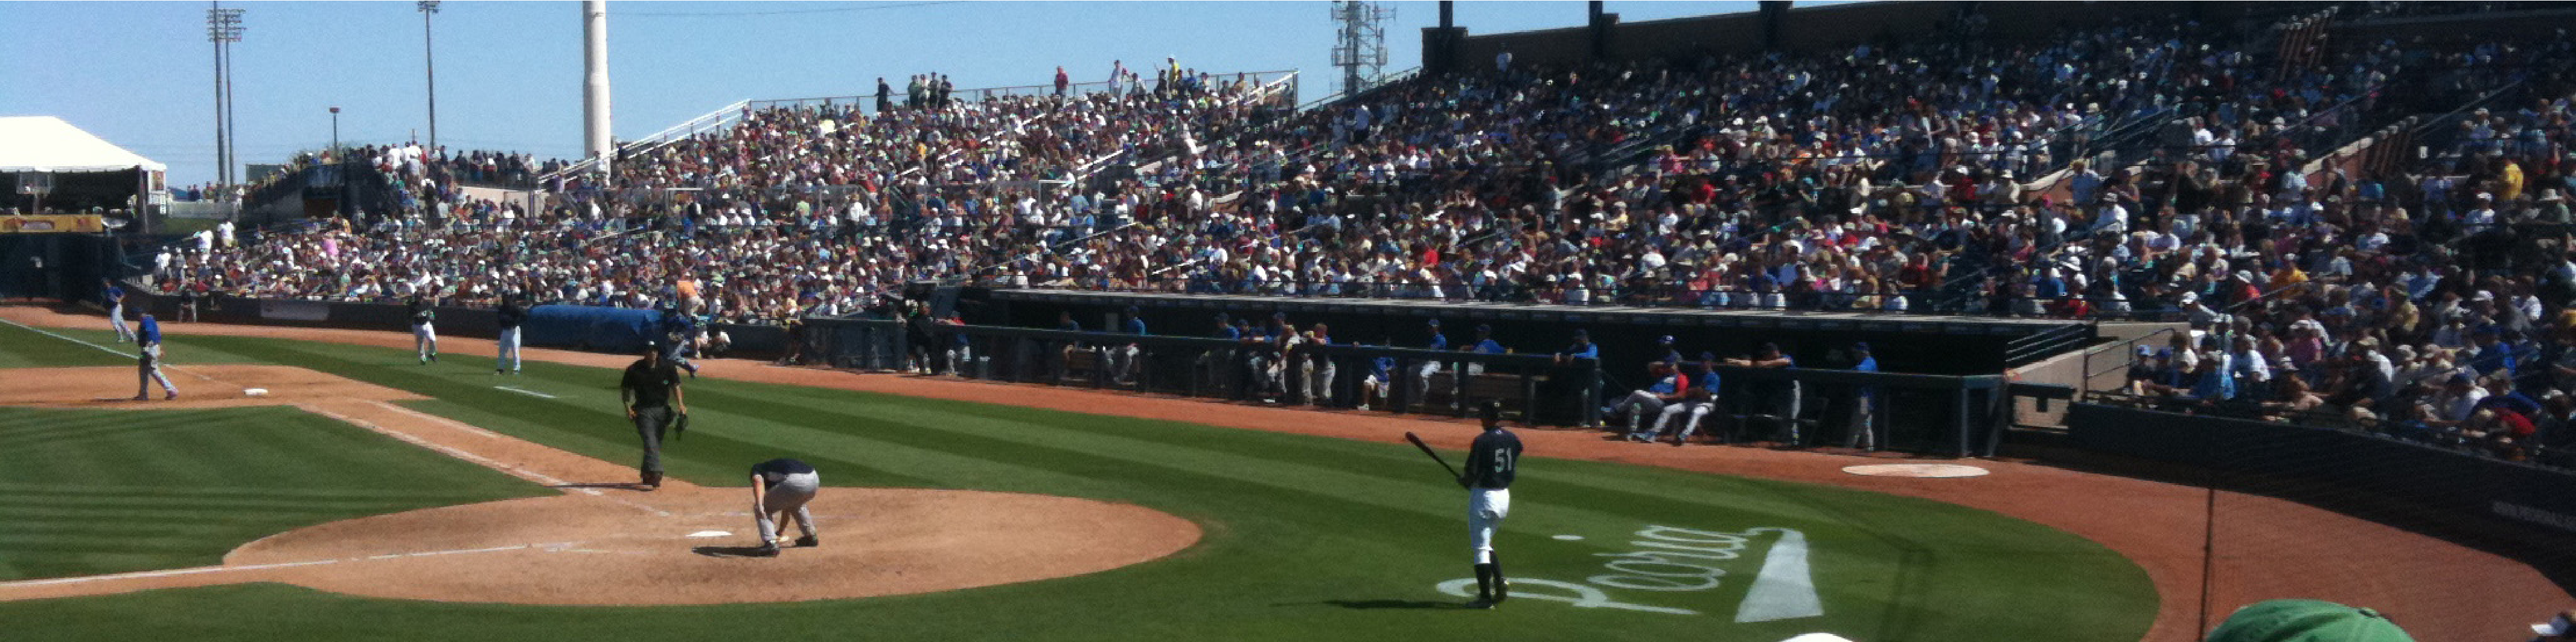
\includegraphics[width=\textwidth]{sampleteaser}
%   \caption{Seattle Mariners at Spring Training, 2010.}
%   \Description{Enjoying the baseball game from the third-base
%   seats. Ichiro Suzuki preparing to bat.}
%   \label{fig:teaser}
% \end{teaserfigure}

%%
%% This command processes the author and affiliation and title
%% information and builds the first part of the formatted document.
\maketitle

\section{Introduction}
1 Graph-structured data is ubiquitous across application domains ranging from chemo- and bioinformatics to image and social network analysis.
2 Graph-structured data is ubiquitous across application domains ranging from chemo- and bioinformatics to image and social network analysis.
3 Graph-structured data is ubiquitous across application domains ranging from chemo- and bioinformatics to image and social network analysis.
4 Graph-structured data is ubiquitous across application domains ranging from chemo- and bioinformatics to image and social network analysis.
5 Graph-structured data is ubiquitous across application domains ranging from chemo- and bioinformatics to image and social network analysis.

\subsection{Present work}
1 Graph-structured data is ubiquitous across application domains ranging from chemo- and bioinformatics to image and social network analysis.
2 Graph-structured data is ubiquitous across application domains ranging from chemo- and bioinformatics to image and social network analysis.
3 Graph-structured data is ubiquitous across application domains ranging from chemo- and bioinformatics to image and social network analysis.
4 Graph-structured data is ubiquitous across application domains ranging from chemo- and bioinformatics to image and social network analysis.
5 Graph-structured data is ubiquitous across application domains ranging from chemo- and bioinformatics to image and social network analysis.

\subsection{Related work}
1 Graph-structured data is ubiquitous across application domains ranging from chemo- and bioinformatics to image and social network analysis.
2 Graph-structured data is ubiquitous across application domains ranging from chemo- and bioinformatics to image and social network analysis.
3 Graph-structured data is ubiquitous across application domains ranging from chemo- and bioinformatics to image and social network analysis.
4 Graph-structured data is ubiquitous across application domains ranging from chemo- and bioinformatics to image and social network analysis.
5 Graph-structured data is ubiquitous across application domains ranging from chemo- and bioinformatics to image and social network analysis.

\section{The CFPQ\_Data collection}
1 We have collected graphs and grammars for analyzing CFPQ algorithms in one place.
2 We have collected graphs and grammars for analyzing CFPQ algorithms in one place.
3 We have collected graphs and grammars for analyzing CFPQ algorithms in one place.
4 We have collected graphs and grammars for analyzing CFPQ algorithms in one place.

\subsection{Graphs and grammars}
1 We have collected graphs and grammars for analyzing CFPQ algorithms in one place.
2 We have collected graphs and grammars for analyzing CFPQ algorithms in one place.
3 We have collected graphs and grammars for analyzing CFPQ algorithms in one place.
4 We have collected graphs and grammars for analyzing CFPQ algorithms in one place.

\textbf{RDF.}
1 We have collected RDF graphs and grammars for analyzing CFPQ algorithms in one place.
2 We have collected RDF graphs and grammars for analyzing CFPQ algorithms in one place.
3 We have collected RDF graphs and grammars for analyzing CFPQ algorithms in one place.
4 We have collected RDF graphs and grammars for analyzing CFPQ algorithms in one place.

\textbf{MemoryAliases.}
1 We have collected MemoryAliases graphs and grammars for analyzing CFPQ algorithms in one place.
2 We have collected MemoryAliases graphs and grammars for analyzing CFPQ algorithms in one place.
3 We have collected MemoryAliases graphs and grammars for analyzing CFPQ algorithms in one place.
4 We have collected MemoryAliases graphs and grammars for analyzing CFPQ algorithms in one place.

\textbf{LUBM.}
1 We have collected LUBM graphs and grammars for analyzing CFPQ algorithms in one place.
2 We have collected LUBM graphs and grammars for analyzing CFPQ algorithms in one place.
3 We have collected LUBM graphs and grammars for analyzing CFPQ algorithms in one place.
4 We have collected LUBM graphs and grammars for analyzing CFPQ algorithms in one place.

\textbf{Synthetic.}
1 We have collected WorstCase graphs and grammars for analyzing CFPQ algorithms in one place.
2 We have collected SparseGraph graphs and grammars for analyzing CFPQ algorithms in one place.
3 We have collected ScaleFree graphs and grammars for analyzing CFPQ algorithms in one place.
4 We have collected FullGraph graphs and grammars for analyzing CFPQ algorithms in one place.

\subsection{Baselines methods (Loaders)}
1 We have made convenient graph and grammar loaders for analyzing CFPQ algorithms in one place.
2 We have made convenient graph and grammar loaders for analyzing CFPQ algorithms in one place.
3 We have made convenient graph and grammar loaders for analyzing CFPQ algorithms in one place.
4 We have made convenient graph and grammar loaders for analyzing CFPQ algorithms in one place.

\subsection{Evaluation methods (Evaluators)}
1 We have made convenient evaluators for analyzing CFPQ algorithms in one place.
2 We have made convenient evaluators for analyzing CFPQ algorithms in one place.
3 We have made convenient evaluators for analyzing CFPQ algorithms in one place.
4 We have made convenient evaluators for analyzing CFPQ algorithms in one place.

\section{Experimental evaluation}
1 We took graphs, grammars and CFPQ algorithms and conducted an experimental analysis.
2 We took graphs, grammars and CFPQ algorithms and conducted an experimental analysis.

\subsection{Datasets}
1 We took RDF, Memoryaliases and WorstCase graphs.
2 We took RDF, Memoryaliases and WorstCase graphs.
3 We took RDF, Memoryaliases and WorstCase graphs.
4 We took RDF, Memoryaliases and WorstCase graphs.

\subsection{Algorithms}
1 We took Matrix and Tensor algorithms.
2 We took Matrix and Tensor algorithms.
3 We took Matrix and Tensor algorithms.
4 We took Matrix and Tensor algorithms.

\subsection{Results and discussion}
1 We got super duper results.
2 We got super duper results.
3 We got super duper results.
4 We got super duper results.

\begin{table}
  \caption{Super Duper Results}
  \label{tab:results}
  \begin{tabular}{cccc}
    \toprule
    Graph & Grammar & Algorithm & Time\\
    \midrule
    RDF&$G_1$&Tensor&$0.001$\\
    RDF&$G_1$&Tensor&$0.001$\\
    RDF&$G_1$&Tensor&$0.001$\\
    RDF&$G_1$&Tensor&$0.001$\\
  \bottomrule
\end{tabular}
\end{table}

\section{Conclusion}
1 CFPQ\_Data is super duper cool!
2 CFPQ\_Data is super duper cool!
3 CFPQ\_Data is super duper cool!
4 CFPQ\_Data is super duper cool!
5 CFPQ\_Data is super duper cool!
6 CFPQ\_Data is super duper cool!

\section{Acknowledgments}
1 We thank everybody who provided datasets for the CFPQ\_Data collection.
2 We thank everybody who provided datasets for the CFPQ\_Data collection.
3 We thank everybody who provided datasets for the CFPQ\_Data collection.
4 We thank everybody who provided datasets for the CFPQ\_Data collection.

%%
%% The acknowledgments section is defined using the "acks" environment
%% (and NOT an unnumbered section). This ensures the proper
%% identification of the section in the article metadata, and the
%% consistent spelling of the heading.
% \begin{acks}
% 1 We thank everybody who provided datasets for the CFPQ\_Data collection.
% 2 We thank everybody who provided datasets for the CFPQ\_Data collection.
% 3 We thank everybody who provided datasets for the CFPQ\_Data collection.
% 4 We thank everybody who provided datasets for the CFPQ\_Data collection.
% \end{acks}

%%
%% The next two lines define the bibliography style to be used, and
%% the bibliography file.
% \bibliographystyle{ACM-Reference-Format}
% \bibliography{sample-base}

%%
%% If your work has an appendix, this is the place to put it.
% \appendix

\end{document}
\endinput
%%
%% End of file `sample-sigconf.tex'.
